\documentclass[12pt]{article}

\usepackage[utf8x]{inputenc} % Включаем поддержку UTF8  
\usepackage[russian]{babel}  % Включаем пакет для поддержки русского языка  
\usepackage{hyperref}        % Для гиперссылок

% Математика
\usepackage{amsmath}         % В т.ч. для матриц
\usepackage{amssymb}

% Прога
\usepackage{etoolbox}
\usepackage{listings}

% Цвета
\usepackage{xcolor}

% Картинки
\usepackage{graphicx}
\graphicspath{ {./images/} }

\newtheorem{property}{Свойство}
\newtheorem{consequence}{Следствие}[property]

\newcommand{\qedsymbol}{\rule{2mm}{2mm}}

\begin{document}

\thispagestyle{empty}
\begin{center}
\textbf{ПРАВИТЕЛЬСТВО РОССИЙСКОЙ ФЕДЕРАЦИИ}

\vspace{5ex}
	
\textbf{Федеральное государственное автономное образовательное учреждение \\ высшего образования \\ <<Национальный исследовательский университет \\ <<Высшая школа экономики>>}
\end{center}
\vspace{5ex}

\begin{center}
    Московский институт электроники и математики им. А.Н. Тихонова  
    
    \vspace{5ex}
    
    Департамент прикладной математики
    
    \vspace{10ex}
    \textbf{Отчёт \\ по лабораторной работе №9 \\ по курсу <<Алгоритмизация и программирование>>}
	\vspace{7ex}

\end{center}

\begin{center} 
\begin{tabular}{| p{0.3\linewidth}| p{0.3\linewidth}| p{0.3\linewidth}|}
 \hline	
ФИО студента & Номер группы & Дата \\  \hline
 & & \\  
Вязов Глеб \newline Дмитриевич & БПМ-231 & 02.03.2024\\  
 & & \\  \hline		
\end{tabular}
\end{center}

\begin{center}
	\vspace{3ex}
	
	\vfill
   
   \normalsize
    
	\textbf{Москва, 2023}
\end{center}

\newpage

%---------------------------------------------------------------------------------

\section*{Задание (вариант №7)}
\begin{enumerate}
	\item Реализовать указанные в варианте алгоритмы сортировки для массива объектов в  соответствии с вариантом. Структура объекта описана в варианте ЛР8. Определить функции сравнения объектов по следующему принципу: приоритет сравнения определяется порядком поля в структуре, т.е. если структурный тип Х содержит (в описании варианта) поля с именами a,b,c,d, то при сравнении двух объектов типа Х надо сравнить поля с именем a, в случае их равенства сравнить поля b и т.д.
	\item Каждый алгоритм сортировки должен поддерживать сортировку в обоих направлениях: по неубыванию и по невозрастанию.
	\item Выбор и запуск требуемого алгоритма и направления сортировки осуществляется через меню на этапе выполнения.
	\item Провести сортировку каждым алгоритмом массивов следующих размеров: 100, 1000, 5000, 10000, 20000, 50000, 100000. Засечь (программно) время сортировки  каждым алгоритмом. По полученным точкам построить графики зависимости времени сортировки от размерности массива для каждого из алгоритмов сортировки на одной оси координат. Полученные графики включить в отчет к работе.
\end{enumerate}


\newpage

%---------------------------------------------------------------------------------

\section*{Решение}\addcontentsline{toc}{section}{Решение}

\lstset{ %
texcl=true,%
language=C,                 % выбор языка для подсветки
basicstyle=\small\sffamily, % размер и начертание шрифта для подсветки кода
numbers=left,               % где поставить нумерацию строк (слева\справа)
numberstyle=\tiny,           % размер шрифта для номеров строк
stepnumber=1,                   % размер шага между двумя номерами строк
numbersep=5pt,                % как далеко отстоят номера строк от подсвечиваемого кода
backgroundcolor=\color{white}, % цвет фона подсветки - используем \usepackage{color}
showspaces=false,            % показывать или нет пробелы специальными отступами
showstringspaces=false,      % показывать или нет пробелы в строках
showtabs=false,             % показывать или нет табуляцию в строках
frame=single,              % рисовать рамку вокруг кода
tabsize=3,                 % размер табуляции по умолчанию равен 2 пробелам
captionpos=t,              % позиция заголовка вверху [t] или внизу [b] 
breaklines=true,           % автоматически переносить строки (да\нет)
breakatwhitespace=false, % переносить строки только если есть пробел
escapeinside={\%*}{*)},   % если нужно добавить комментарии в коде
inputencoding=utf8x,
extendedchars=\true
}

\begin{lstlisting}[label=structs.h, caption=structs.h]
#ifndef HW9_STRUCTS_H
#define HW9_STRUCTS_H

# define N 50

struct Sportsmen {
    char fio[N];  // ФИО
    int age;      // Возраст
    int height;   // Рост
    int weight;   // Вес
    char type[N]; // Вид спорта
    char rank[N]; // Спотртивное звание
};

void printSportsmen(struct Sportsmen sportsmen);
void printArrayOfSportsmen(struct Sportsmen sportsmen[], int len);
int compareSportsmens(struct Sportsmen sportsmen1, struct Sportsmen sportsmen2);
struct Sportsmen* generateSportmens(int count);
int random(int min, int max);

#endif
\end{lstlisting} 

\newpage

\begin{lstlisting}[label=sorting.c, caption=sorting.c]
#include <stdlib.h>
#include "repository.c"

/*
 * Для всех сортировок: параметр ascending отвечает за порядок сортировки
 * Если ascending = 1, то сортировка по возрастанию
 * Если ascending = -1, то сортировка по убыванию
 */

// Сортировка вставками. Время: O(n**2). Память: O(1)
void insertSort(struct Sportsmen array[], int len, int ascending) {
    struct Sportsmen value;
    int j;

    for (int i=1; i<len; i++) {
        value = array[i];

        for (j=i-1; j >= 0; j--) {
            if (ascending*compareSportsmens(array[j], value) == 1) {
                array[j+1] = array[j];
            } else {
                break;
            }
        }

        array[j+1] = value;
    }
}

// Вспомогательная функция для сортировки слиянием
void merge(struct Sportsmen array[], int l, int m, int r, int ascending) {
    int len1 = m - l + 1;
    int len2 = r - m;
    struct Sportsmen* left = calloc(len1, sizeof(struct Sportsmen));  // [l, m]
    struct Sportsmen* right = calloc(len2, sizeof(struct Sportsmen)); // [m+1, r]
    int i = l, i1=0, i2=0; // i -- индекс для array, i1 -- индекс для left, i2 -- индекс для right

    // Заполняем левые и правые части массивов элементами исходного
    for (int k=l; k<=m; k++) {
        left[k-l] = array[k];
    }
    for (int k=m+1; k<=r; k++) {
        right[k-(m+1)] = array[k];
    }

    // Алгоритм сортировки
    while (i1 < len1 && i2 < len2) {
        if (ascending*compareSportsmens(right[i2], left[i1]) == 1) { // right[i2] >= left[i1]
            array[i] = left[i1];
            i1++;
        } else {
            array[i] = right[i2];
            i2++;
        }
        i++;
    }

    // Один из индексов может не дойти до конца
    while (i1 < len1) {
        array[i] = left[i1];
        i++;
        i1++;
    }

    while (i2 < len2) {
        array[i] = right[i2];
        i++;
        i2++;
    }

    free(left);
    free(right);
}

// Сортировка слиянием. Время: O(nlog n). Память: O(n)
// Сортируемый диапозон: array[l], ..., array[r] (все границы включены)
void mergeSort(struct Sportsmen array[], int l, int r, int ascending) {
    if (r <= l) {
        return;
    }

    int m = l + (r - l) / 2;
    mergeSort(array, l, m, ascending);
    mergeSort(array, m+1, r, ascending);
    merge(array, l, m, r, ascending);
}

// Вспомогательная функция для быстрой сортировки
// Меняет местами значения a и b
void swap(struct Sportsmen* a, struct Sportsmen* b) {
    struct Sportsmen temp = *a;
    *a = *b;
    *b = temp;
}

// Вспомогательная функция для быстрой сортировки
// Возвращает индекс "разделяющего" элемента
// Слева от "разделяющего" элемента находятся элементы, которые меньше его, а справа, которые больше
int partition(struct Sportsmen array[], int l, int r, int ascending) {
    struct Sportsmen pivot = array[l];
    int i = l, j = r;

    while (i < j) {
        if (ascending == 1) {
            // Находим индекс элемента, который больше pivot: pivot >= array[i]
            while (compareSportsmens(pivot, array[i]) == 1 && i <= r - 1) { i++; }
            // Находим индекс элемента, который меньше pivot: array[j] >= pivot
            while (compareSportsmens(array[j], pivot) == 1 && j >= l + 1) { j--; }
        } else {
            // Находим индекс элемента, который меньше pivot: array[i] >= pivot
            while (compareSportsmens(array[i], pivot) == 1 && i <= r - 1) { i++; }
            // Находим индекс элемента, который больше pivot: pivot >= array[j]
            while (compareSportsmens(pivot, array[j]) == 1 && j >= l + 1) { j--; }
        }

        if (i < j) {
            swap(&array[i], &array[j]);
        }
    }
    // Возвращаем на место разделяющий элемент
    swap(&array[l], &array[j]);
    return j;
}

// Быстрая сортировка. Время: O(nlog n). Память: O(1)
void quickSort(struct Sportsmen array[], int l, int r, int ascending) {
    if (l >= r) {
        return;
    }

    // Выбираем разделяющий элемент
    int partitionIndex = partition(array, l, r, ascending);

    quickSort(array, l, partitionIndex - 1, ascending);
    quickSort(array, partitionIndex + 1, r, ascending);
}
\end{lstlisting} 

\newpage

\begin{lstlisting}[label=repository.c, caption=repository.c]
#include <stdio.h>
#include <stdlib.h>
#include <string.h>
#include "structs.h"

#define LEN_FIOS 18
#define LEN_TYPES 15
#define LEN_RANKS 14

const char FIOS[LEN_FIOS][N] = {
        "Иван Иванов", "Павел Артемьев", "Емельяненко Федор",
        "Арнольд Шварцнегер", "Луговой Александр", "Сарычев Кирилл", "Джулиус Мэддокс",
        "Тайсон Майк", "Попович Алеша", "Муромец Илья", "Добрыня Никитич", "Ронни Колман",
        "Цзю Константин", "Хабиб", "Конор Макгрегор", "Фишер Роберт", "Карякин Сергей",
        "Магнус Карлсен"
};
const char TYPES[LEN_TYPES][N] = {
        "Тяжелая атлетика", "ММА", "Бокс", "Самбо", "Дзюдо", "Пауэрлифтинг",
        "Легкая атлетика", "АРБ", "Кикбоксинг", "Тайский бокс", "БЖЖ",
        "Бодибилдинг", "Шахматы", "Водное поло", "Плавание"
};
const char RANKS[LEN_RANKS][N] = {
        "ЧМ", "МСМК", "ЗМС", "МС", "КМС", "1 взрослый разряд", "2 взрослый разряд",
        "3 взрослый разряд", "1 юношеский разряд", "2 юношеский разряд", "3 юношеский разряд",
        "Любитель", "Просто за ЗОЖ", "Олимпиец"
};

// Вывод спортсмена в консоль
void printSportsmen(struct Sportsmen sportsmen) {
    printf("%s, %d, %d, %d, %s, %s\n", sportsmen.fio, sportsmen.age, sportsmen.height, sportsmen.weight,
           sportsmen.type, sportsmen.rank);
}

// Вывод массива спортсменов в консоль
void printArrayOfSportsmen(struct Sportsmen sportsmen[], int len) {
    for (int i=0; i<len; i++) {
        printSportsmen(sportsmen[i]);
    }
    printf("\n");
}

// Функция сравнивает двух спортсменов
// Возвращает 1, если sportsmen1 >= sportsmen2
// Возвращает -1, если sportsmen1 < sportsmen2
int compareSportsmens(struct Sportsmen sportsmen1, struct Sportsmen sportsmen2) {
    // Сравнение ФИО
    int compareFio = strcmp(sportsmen1.fio, sportsmen2.fio);
    if (compareFio > 0) {
        return 1;
    } else if (compareFio < 0) {
        return -1;
    }

    // Сравнение возраста
    if (sportsmen1.age > sportsmen2.age) {
        return 1;
    } else if (sportsmen1.age < sportsmen2.age) {
        return -1;
    }

    // Сравнение роста
    if (sportsmen1.height > sportsmen2.height) {
        return 1;
    } else if (sportsmen1.height < sportsmen2.height) {
        return -1;
    }

    // Сравнение веса
    if (sportsmen1.weight > sportsmen2.weight) {
        return 1;
    } else if (sportsmen1.weight < sportsmen2.weight) {
        return -1;
    }

    // Сравнение вида спорта
    int compareType = strcmp(sportsmen1.type, sportsmen2.type);
    if (compareType > 0) {
        return 1;
    } else if (compareType < 0) {
        return -1;
    }

    // Сравнение спортивного звания
    int compareRank = strcmp(sportsmen1.rank, sportsmen2.rank);
    if (compareRank > 0) {
        return 1;
    } else if (compareRank < 0) {
        return -1;
    }

    // Объекты равны
    return 1;
}

// Генерация пвесво-рандомного числа из диапозона [min; max]
int random(int min, int max) {
    return min + rand()%(max-min);
}

// Функция генерирует массив из спортсменов длиной count
struct Sportsmen* generateSportmens(int count) {
    struct Sportsmen* sportsmens = calloc(count, sizeof(struct Sportsmen));

    for (int i=0; i<count; i++) {
        struct Sportsmen sp;
        strcpy(sp.fio, FIOS[random(0, LEN_FIOS-1)]);
        sp.age = random(18, 60),
        sp.height = random(160, 210),
        sp.weight = random(50, 170),
                strcpy(sp.type, TYPES[random(0, LEN_TYPES-1)]);
        strcpy(sp.rank, RANKS[random(0, LEN_RANKS-1)]);

        sportsmens[i] = sp;
    }
    return sportsmens;
}
\end{lstlisting} 

\newpage

\begin{lstlisting}[label=hw9.c, caption=hw9.c]
#include <stdio.h>
#include <windows.h>
#include "sorting.c"

int main() {
    // Меняем кодировку на UTF-8, чтобы можно было писать на русском
    SetConsoleOutputCP(CP_UTF8);
    // Ввод переменных. Дружественный интерфейс
    printf("Выполнил задание: Вязов Глеб. Группа: БПМ231\n");

    int count, type_sorting, asc;

    printf("Введите длину массива, который будем сортировать: ");
    scanf("%d", &count);
    struct Sportsmen* sportsmens = generateSportmens(count);
    printArrayOfSportsmen(sportsmens, count);
    printf("Выберите алгоритм сортировки:\n"
           "1. Сортировка вставками\n"
           "2. Сортировка слиянием\n"
           "3. Быстрая сортировка\n");
    scanf("%d", &type_sorting);
    printf("Выберите направление сортировки:\n"
           "По возврастанию -- 1\n"
           "По убыванию -- -1\n");
    scanf("%d", &asc);
    switch (type_sorting) {
        case 1:
            insertSort(sportsmens, count, asc);
            break;
        case 2:
            mergeSort(sportsmens, 0, count-1, asc);
            break;
        case 3:
            quickSort(sportsmens, 0, count-1, asc);
            break;
    }
    printArrayOfSportsmen(sportsmens, count);
    free(sportsmens);
}
\end{lstlisting} 

\newpage

\begin{lstlisting}[label=timing.c, caption=timing.c]
#include <time.h>
#include <windows.h>
#include "sorting.c"

const int sizes[] = {100, 1000, 5000, 10000, 20000, 50000, 100000};

int main() {
    // Меняем кодировку на UTF-8, чтобы можно было писать на русском
    SetConsoleOutputCP(CP_UTF8);

    double timeSpent;
    printf("Сортировка вставками:\n");
    for (int i=0; i<7; i++) {
        struct Sportsmen* sportsmens = generateSportmens(sizes[i]);

        clock_t begin = clock();
        insertSort(sportsmens, sizes[i], 1);
        clock_t end = clock();
        timeSpent = (double)(end - begin) / CLOCKS_PER_SEC;

        printf("Длина массива = %5d, время работы = %10.4lf секунд\n", sizes[i], timeSpent);
    }

    printf("\nСортировка слиянием:\n");
    for (int i=0; i<7; i++) {
        struct Sportsmen* sportsmens = generateSportmens(sizes[i]);

        clock_t begin = clock();
        mergeSort(sportsmens, 0, sizes[i]-1, 1);
        clock_t end = clock();
        timeSpent = (double)(end - begin) / CLOCKS_PER_SEC;

        printf("Длина массива = %5d, время работы = %10.4lf секунд\n", sizes[i], timeSpent);
    }

    printf("\nБыстрая сортировка:\n");
    for (int i=0; i<7; i++) {
        struct Sportsmen* sportsmens = generateSportmens(sizes[i]);

        clock_t begin = clock();
        quickSort(sportsmens, 0, sizes[i]-1, 1);
        clock_t end = clock();
        timeSpent = (double)(end - begin) / CLOCKS_PER_SEC;

        printf("Длина массива = %6d, время работы = %10.4lf секунд\n", sizes[i], timeSpent);
    }

    return 0;
}
\end{lstlisting} 

\newpage

%---------------------------------------------------------------------------------

\section*{Тестирование}
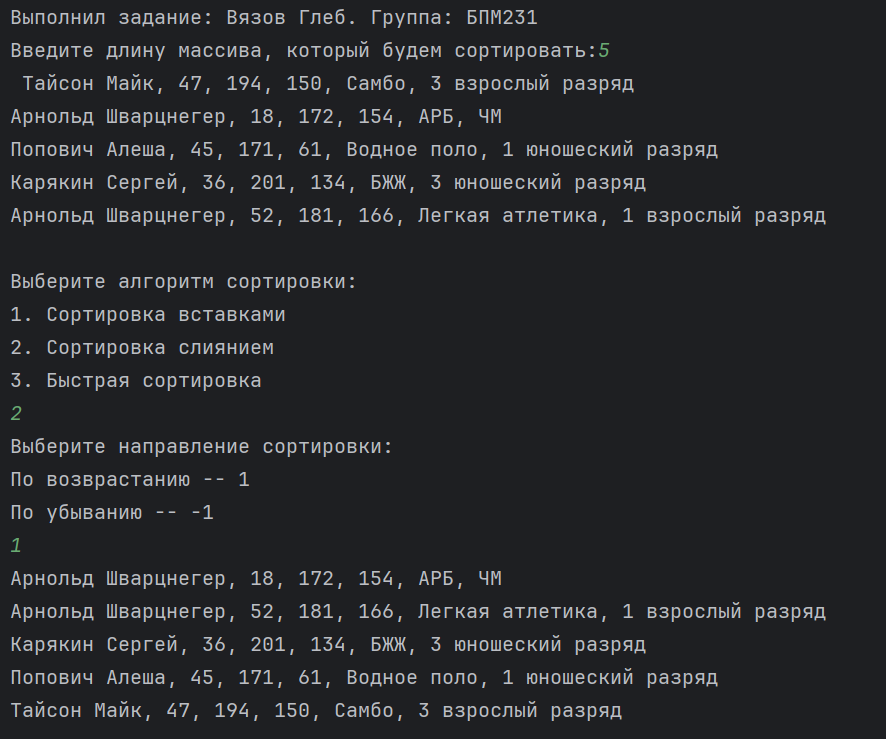
\includegraphics[scale=0.8]{img1}

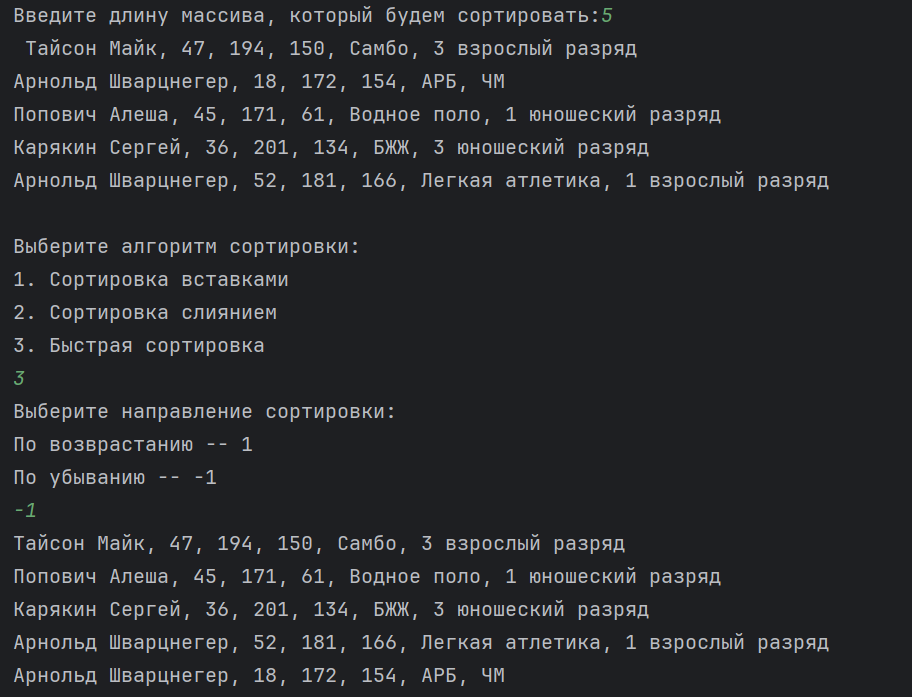
\includegraphics[scale=0.8]{img2}

\end{document}
